\documentclass[12pt, %
openright, 
oneside, %
%twoside, %TCC: Se seu texto tem mais de 100 páginas, descomente esta linha e comente a anterior
a4paper,    %
%english,   %
brazil]{facom-ufu-abntex2}

\usepackage{graphicx}
\graphicspath{{figuras/}{pictures/}{Images/}{./}} % where to search for the images

\newcommand{\blue}[1]{\textcolor{blue}{#1}}
\newcommand{\red}[1]{\textcolor{red}{#1}}


\autor{Paulo Kiyoshi Oyama Filho} %TCC
\data{2024}
\orientador{Pedro Franklin} %TCC
%\coorientador{Algum?} %TCC

% ---
% Informações de dados para CAPA e FOLHA DE ROSTO
% ---


\hypersetup{pdfkeywords={palavra 1}{palavra 2}{palavra 4}{palavra 4}{palavra 5}} %TCC

\begin{document}
\frenchspacing

% ----------------------------------------------------------
% ELEMENTOS PRÉ-TEXTUAIS
% ----------------------------------------------------------
%\pretextual
\imprimircapa
\imprimirfolhaderosto


% ---
% Inserir folha de aprovação
% ---
%
% \includepdf{folhadeaprovacao_final.pdf} %TCC: depois de aprovado o trabalho, descomente esta linha e comente o próximo bloco para incluir scan da folha de aprovação.
%
\begin{folhadeaprovacao}
  \graphicspath{ {./Images/} }

  \begin{center}
    {\ABNTEXchapterfont\large\imprimirautor}

    \vspace*{\fill}\vspace*{\fill}
    {\ABNTEXchapterfont\bfseries\Large\imprimirtitulo}
    \vspace*{\fill}

    \hspace{.45\textwidth}
    \begin{minipage}{.5\textwidth}
      \imprimirpreambulo
    \end{minipage}%
    \vspace*{\fill}
  \end{center}

  Trabalho aprovado. \imprimirlocal, 01 de novembro de 2016: %TCC:

  \assinatura{\textbf{\imprimirorientador} \\ Orientador}
  \assinatura{\textbf{Professor}}% \\ Convidado 1} %TCC:
  \assinatura{\textbf{Professor}}% \\ Convidado 2} %TCC:
  %\assinatura{\textbf{Professor} \\ Convidado 3}
  %\assinatura{\textbf{Professor} \\ Convidado 4}

  \begin{center}
    \vspace*{0.5cm}
    {\large\imprimirlocal}
    \par
    {\large\imprimirdata}
    \vspace*{1cm}
  \end{center}

\end{folhadeaprovacao}
% ---


%%As seções dedicatória, agradecimento e epígrafe não são obrigatórias.
%%Só as mantenha se achar pertinente.

% ---
% Dedicatória
% ---
%\begin{dedicatoria}
%   \vspace*{\fill}
%   \centering
%   \noindent
%   \textit{Dedico a \lipsum[10]}  %TCC:
%   \vspace*{\fill}
%\end{dedicatoria}
% ---

% ---
% Agradecimentos
% ---
%\begin{agradecimentos}
%Agradeço a \lipsum[30]. %TCC:
%\end{agradecimentos}
% ---

% ---
% Epígrafe
% ---
%\begin{epigrafe}
%    \vspace*{\fill}
%	\begin{flushright}
%		\textit{``Alguma citação que ache conveniente? \lipsum[10]''} %TCC:
%	\end{flushright}
%\end{epigrafe}
% ---



\begin{resumo} %TCC:
  Segundo a \citeonline[3.1-3.2]{NBR6028:2003}, o resumo deve ressaltar o
  objetivo, o método, os resultados e as conclusões do documento. A ordem e a extensão
  destes itens dependem do tipo de resumo (informativo ou indicativo) e do
  tratamento que cada item recebe no documento original. O resumo deve ser
  precedido da referência do documento, com exceção do resumo inserido no
  próprio documento. (\ldots) As palavras-chave devem figurar logo abaixo do
  resumo, antecedidas da expressão Palavras-chave:, separadas entre si por
  ponto e finalizadas também por ponto.

  \vspace{\onelineskip}

  \noindent
  \textbf{Palavras-chave}: Até, cinco, palavras-chave, separadas, por, vírgulas. %TCC:
\end{resumo}

% ---
% inserir lista de ilustrações
% ---
\pdfbookmark[0]{\listfigurename}{lof}
\listoffigures*
\cleardoublepage
% ---

% ---
% inserir lista de tabelas
% ---
\pdfbookmark[0]{\listtablename}{lot}
\listoftables*
\cleardoublepage
% ---



% ---
% inserir lista de abreviaturas e siglas
% ---
\begin{siglas} %TCC:
  \item[Fig.] Area of the $i^{th}$ component
  \item[456] Isto é um número
  \item[123] Isto é outro número
  \item[Zézão] este é o meu nome
\end{siglas}
% ---

%% ---
%% inserir lista de símbolos, se for adequado ao trabalho. %TCC:
%% ---
%\begin{simbolos}
%  \item[$ \Gamma $] Letra grega Gama
%  \item[$ \Lambda $] Lambda
%  \item[$ \zeta $] Letra grega minúscula zeta
%  \item[$ \in $] Pertence
%\end{simbolos}
%% ---

% ---
% inserir o sumario
% ---
\pdfbookmark[0]{\contentsname}{toc}
\tableofcontents*
\cleardoublepage
% ---





% ----------------------------------------------------------
% ELEMENTOS TEXTUAIS
% ----------------------------------------------------------
\textual


% ----------------------------------------------------------
% Introdução
% ----------------------------------------------------------

\chapter[Introdução]{Introdução}
%TCC:


O desenvolvimento da Internet, dos dispositivos móveis e de diversas formas de entretenimento juntamente com a grande dispersão destes entre as pessoas, causaram um impacto substancial no avanço das formas de lazer já estabelecidas e criação de novas, levando a um aumento de conteúdos inéditos, novos temas e estilos. Na música, pode-se observar a ascensão dos \textit{streamings} de áudio como uma ferramenta do dia a dia popular, como forma de lazer, cultura e ensino, propondo conteúdos musicais de vários artistas, lugares e épocas  para variados públicos em abundância de forma rápida e assertiva.


"\textit{Music is subjective and universal.}" \cite{song2012survey}. Diferentes gostos, idades e personalidades acabam por modificarem as escolhas musicais de um indivíduo, por consequência, há a necessidade de algoritmos que consigam acompanhar a evolução dos conteúdos midiáticos e recomendar assuntos que possam encaixar-se ao público, a época e aos diversos tipos musicais que nascem a cada momento em diferentes lugares do mundo. Tendo em vista essa forma de expressão essencialmente humana que pode ser encontrada desde os tempos primitivos e para alguns sendo até mesmo uma forma de tratamento de doenças, como argumenta Michael H. Thaut (\citeyear{thaut2015music}) em seu artigo.


Por conta disso, muitos autores têm empenhado-se para conseguir construir e desenvolver algoritmos que possibilitam uma eficiente experiência para os usuários, como os trabalhos de \cite{de2009se} e \cite{monteirosistema}, \cite{aliaga2019desenvolvimento}
que promovem a criação de sistemas que possam comportar a grande quantidade de dados e usuários em ambientes de música sejam eles individuais ou compartilhados. Ademais, há outros artigos que explicitam as dificuldades, possíveis caminhos e estratégias na criação deste tipo de produto dando uma percepção abrangente do assunto e elucidando possíveis dúvidas, como os \textit{surveys} \cite{de2009se} e \cite{ko2022survey}.


Para tanto, o trabalho de conclusão de curso busca entender as dificuldades referentes a área de indicação de músicas, haja vista a diversidade de estilos melodias e variados gostos de cada indivíduo, e por meio dos métodos matemáticos para aprendizado de máquina (não supervisionado e supervisionado) e de um conjunto de dados criados a partir de API's públicas conseguir organizar, classificar e categorizar as informações com base em cada usuário ou grupo, de tal forma que, ao final possa originar sistemas de recomendação criados com base em difentes algoritmos aprendidos ao longo do curso. Por final, possibilitando não somente o entendimento computacional mas também o pensamento matemático em uma aplicação real e importante no cotidiano popular.


Finalmente, técnicas de pré processamento, como balaceamento de classe (\textit{random sampling, oversampling e undersampling}), serão usados para filtrar os dados escolhidos previamente, após isso o estudo usará das linguagens \textit{R} e \textit{Python} para conseguir implementar métodos matemáticos como \textit{Naive Bayes e KNN}. E, por meio dos resultados gerados inferir a qualidade dos dados considerando alguma métrica (\textit{Gain Ratio, Gini Index}) juntamente com a possibilidade de discutir possíveis melhorias, abordagens mais suaves sobre os problemas encontrados na metodologia e a expectativa de trabalhos futuros.


\chapter{Fundamentação Teórica}
%TCC:
A teoria pode da monografia pode ser divida em duas fases, sistemas de recomendação e algoritmos de aprendizado de máquina.

\section{Sistemas de Recomendação}


Sistemas de Recomendação são ferramentas que ajudam ao consumidor achar alguns conteúdos, produtos ou serviços agregando e analisando sugestões de outros usuários ou produtos previamente avaliados \cite{park2012literature}  haja vista o seu impacto causado pela propagação de dispositivos tecnológicos assim como aplicativos de fácil acesso a diversas formas de entretenimento que acabam por dificultar uma recomendação eficiente em meio a uma infinidade de possibilidades que o cliente pode optar.
A música é uma parte essencial do cotidiano popular sendo um atividade mais frequente do que todas as outras como mostra  pesquisas anteriores \cite{song2012survey}, sendo uma parte essencial da cultura humana e podendo ser usada até mesmo para cura de doenças, por conta dissos sistemas de recomendação que sejam robustos e eficientes para conseguir dar uma resposta rápida e excelente mediante ao conjunto abundante de possibilidades presentes fazem-se necessários.

Em um sistema de recomendação ideal ela conseguiria recomendar músicas personalizadas para diferentes usuários da melhor maneira, em termos formais, seja \textit{C} o conjunto de todos os usuários e \textit{S} o conjunto de todas as possíveis recomendações, o espaço \textit{S} pode conter milhares ou milhões de items possíveis (músicas, livros, filmes). Seja \textit{u} uma função de utilidade que mensura a utilidade de um item \textit{s} para um usuário \textit{c}, por fim procuramos no espaço um par ordenado de (usuário, item) que seja o mais eficiente para a função \textit{u}, em outras palavras, que seja a melhor recomendação possível \cite{adomavicius2005toward}.

\begin{equation}
  \forall \, c \in C, \textit{s} \in \textit{S},  \ s'_{c} = arg \, max \, u(c,s)
\end{equation}


Portanto, diversos tipos de abordagem para o mesmo problema foram desenvolvidos, os mais comuns são os modelos baseados em conteúdo, os filtros colaborativos e os híbridos são também os mais velhos, o primeiro baseia-se na habilidade do sistema de reconhecer por meio de assuntos classificados anteriormente pelo usuário um potencial novo conteúdo que pode ser do agrado dele, o segundo é semelhante ao estilo de recomendação mais trivial, o boca a boca, no qual pessoas próximas a você acabam por recomendar músicas que elas ouviram e gostaram, ou seja, por meio da classificação de terceiros com alta proximidade do usuário alvo, o sistema reconhece semelhanças e indica materiais consumidos em comum pela vizinhança, o terceiro é uma mistura de um ou mais protótipos de recomendação no qual a fraqueza de um modelo pode ser atenuado ou removido quando mesclado com um outro amostra \cite{adomavicius2005toward}.

Com o passar do tempo e a evolução tecnológica, outros tipos de abordagem surgiram para tentar superar as fraquezas dos anteriores, sendo eles recuperação de informação por metadados, no qual por meio das características fundamentais do som, por exemplo, timbre, volume, acústico, outros sons parecidos serão aconselhados. Além deste, o modelo baseado em contexto propõe-se a analisar informações sobre o momento do dia, a atividade que será realizada enquanto consumindo o material recomendado ou a finalidade do conteúdo, por exemplo, uma playlist para ouvir na academia ou dirigindo certamente seriam diferentes em estilos e características musicais, então por meio do contexto busca-se prever o tipo de músicas que melhor adéquam-se a situação e, por fim, os modelos baseados em emoção, como o nome sugere o sistema usa-se do sentimento do usuário para conseguir prescrever uma série de conteúdos que melhor adequariam-se ao humor dele buscando criar um sentimento de empatia ou até mesmo conforto para com o ouvinte \cite{song2012survey}.

\section{Algoritmos de Aprendizado de Máquina}


Desde que os computadores foram criados, foi conjecturado a possibilidade deles conseguirem pensar, construir e falarem por si só de tal forma que não precisaria haver instruções claras e objetivas, em vista dessa esperança de sustentar esse desejo ancestral e profundo muitos caminhos tiveram que ser pavimentados.

Historicamente, o termo aprendizado de máquina (\textit{machine learning}) tem origem dos trabalhos do psicólogo Frank Rosenblatt da universidade da Cornell, que baseou seus estudos sobre o sistema nervoso humano para construir um sistema que reconhece-se o alfabeto de Rosenblatt, seu nome foi "Perceptron" o qual tornou-se o protótipo das redes neurais artificiais. Seu desenvolvimento assemelhou-se ao aprendizado de animais e seres humanos na psicologia, contudo havia algumas limitações intrínsecas a sua implementação que o impedia de atingir todos os escopos. Por conta da criação dessa nova técnica que representava o cumprimento de um antigo sonho, muitos pesquisadores ficaram entusiasmados e propuseram-se a tentar resolver as limitações do primeiro assim como melhorá-lo ou desenvolvê-lo em áreas antes inexploradas, e com o engatinhar dessa área, as grandes empresas observaram que certos problemas que as ténicas desenvolvidas solucionavam acabavam por encaixar em problemas no cotidiano do mercado ocasionando uma massiva onda de investimentos na esperança de uma medicina para dores antigas \cite{fradkov2020early}.

Entretanto, pela falta de poder compucitacional, assim como a falta de disponibilidade de dados e hardware equivalentemente eficiente para que essas ténicas pudessem ser estudadas, implementadas e desenvolvidas, um desânimo instarou-se por parte das instituições e empresas já que era inviável os muitos investimentos e poucos retornos, gerando por fim um período de desaceleração na área de aprendizado de máquina nomeado de \textit{Cold Winter}. Seu renascimento começou no início do século XXI causado pelo início da era de \textit{BigData}, assim como uma explosão no poder computacional marcado pelo paralelismo computacional, uma grande mudança nas \textit{GPU}'s da NVIDIA e pela acessibilidade do hardware dada pelo seu barateamento em mercado, essa período tem sido nomeado como "\textit{The Gold Rush of Machine Learning}" \cite{fradkov2020early}.

Uma das grandes características da \textit{BigData} é sua grande disponibilidade de dados públicos, entretanto muitas das informações presentes na Internet não são bem estruturadas e seu tratamento muita das vezes é inviável, em vista disso, as ténicas de aprendizionado não supervisionado tem crescido exponecialmente buscando reparar e desenvolver a acurácia das arquétipos vigentes, seus objetivos divergem, indo desde visualização de dados em altas dimensões passando por reconhecimento de imagens e indo até previsões meterológicas, ou seja, problemas do cotidiano que sua resolução não são fáceis causados por múltiplas variáveis e saídas imprevisíveis.

Ainda sim, as técnicas de aprendizado máquinas permanecem dividas em duas grandes áreas, as supervisionadas e as não supervisionadas, o primeiro corresponde a um sistema que consegue verificar sua saída, ou seja, a saída esperada já é conhecida, e podem ser englobadas em duas grandes categorias, as de regressão e as de classificação \cite{soofi2017classification}. Por fim, o segundo corresponde a um modelo sem qualquer tipo de classificação, ou seja, a saída esperada não é dada, o protótipo busca estabelecer padrões estatísticos para gerar classes as quais para cada valor do conjunto de entrada pertença a uma delas.

Um fato importante é que todas tem sua especificidade, uma função de medição de desempenho diferente e uma hipotése de resolução diferente, seu uso e arquitetura dependem do problema abordado. Alguns aprendizados supervisionados são baseados em instâncias, outros são baseados em técnicas estatísticas e alguns são baseados em lógica \cite{soofi2017classification}. No primeiro temos o exemplo do \textit{K-Nearest Neighbors(KNN)}, a qual tenta classificar uma dado valor levando em conta seus vizinhos, tendo como premissa que aqueles que estão perto um do outro terão caracterísitcas em comum, sendo usadas no reconhecimento facial, reconhecimento da folha de plantas e, como a monografia propõe, conseguir recomendar músicas através do metadado individual delas. Ademais, no segundo temos exemplos como \textit{Naive Bayes}, \textit{Bayesian Network}, \textit{Monte Carlos}, \textit{Markov Chain}, sendo usados para comunicação da internet e telecomunicações, teste de ambientes físicos complexos e verificação de assinatura, e ao final modelos como a \textit{Decision Tree(ID3)} sendo usadas na predição da perfomance de estudantes, classificação da capacidade de terra e detectação de fraude.



\chapter{Trabalhos Relacionados}


Mediante a abundância de dificuldades para o tema de Sistemas de Recomendação muitos autores dispuseram-se a tentar explicar as suas melhores formas de resolução, desde usar metadados da música para conseguir dar mais robustez ao modelo até entender as emoções da pessoa que está consumindo o conteúdo para assim aumentar a  sua acurácia, outros ainda escreveram pesquisas nos quais testavam a eficiência e resultados dos modelos teorizados previamente.

Uma das \textit{surveys} pioneiras nesse assunto foi a dos pesquisadores Gediminas Adomavicius e Alexander Tuzhilin publicada na revista do IEEE chamada de "\textit{Towards the Next Generation of Recommender Systems: A Survey of the State-of-the-Art and Possible Extensions}"  no ano de 2005 \cite{adomavicius2005toward}. Neste artigo os autores propõem 3 tipos de arquitetura para conseguir resolver o problema juntamente com suas falhas inerentes, sendo estes, o modelo baseado em conteúdo, em filtragem colaborativa e o híbrido. A pesquisa busca explicar cada uma delas e qual função heurística (\textit{Knn},\textit{Clustering} e outros) é melhor para elas, por ter tamanha quantidade de instruções essa \textit{survey} pode ser aplicada na parte musical para construir modelos que encaixam-se na realidade do ouvinte.

Contudo, os problemas desses modelos tornam-os limitados não conseguindo abranger todas as necessidades do usuário, em vista disso, após 7 anos, os pesquisadores Yading Song, Simon Dixon, and Marcus Pearce publicaram uma \textit{survey} chamada de "\textit{A Survey of Music Recommendation Systems and Future Perspectives}". Nela propuseram outros 3 modelos além dos já citados, no qual discutiam levar em conta o contexto, a emoção e os metadados da música, recomendando assim músicas que assemelham-se estruturalmente com o mesmo volume, mesma duração, mesmo timbre e outros \cite{song2012survey}.

Por meio das pesquisas feitas pelas \textit{surveys}, muitos trabalhos foram inspiradoes, um deles foi o William Kraemer Aliaga, escrito em 2019, com o tema "Desenvolvimento de um sistema de recomendação musical sensível ao contexto". Nele o autor buscou criar um sistema de recomendação utilizando-se da ajuda do próprio ouvinte, no contexto de correr, trabalhar, relaxar, estudar e dirigir podendo ter músicas do Brasil ou dos Estados Unidos. Além disso, em sua metodologia ele faz um pré processamento retirando dados da API pública da ferramenta de música conhecida como \textit{Spotify} e depois usando o método de \textit{KNN} para conseguir recomendar músicas parecidas, por fim, o autor concluiu que as recomendações contextualizados possuem maior \textit{recall} do que as recomendações normais \cite{aliaga2019desenvolvimento}. Sua monografia distingue-se das outras por usar estratégias e abordagens interessantes, desde a forma de conseguir bases de dados de plataforma já existentes e consolidadas com uma API pública até o treinamento por meio do algoritmo de \textit{KNN} e métricas de performance como semelhança de cossenos.

Ao final, uma outra monografia semelhante a anterior foi a dos estudantes Ariel Godinho e Felipe Vasconcelos, escrita em 2018 e nomeada de "Recomendação Musical para Grupos Baseada em Modelo Híbrido". Nele os escritores construíram um sistema de recomendação nomeada de \textit{Ideal Music} por meio de um algoritmo diferente dos demais, o \textit{K-Means}, sua abordagem para constuir o conjunto de dados foi igual a monografia anterior entretanto com uma camada adicional um banco de dados para conseguir diminuir a taxa de requisição de API's e ter uma maior rapidez de resposta ao final\cite{godinhorecomendaccao}, sendo uma ideia que pode ser replicada neste trabalho de conclusão de curso para não excer a taxa limite de requisições suportadas pela plataforma.



\chapter{Método}
%TCC:

O trabalho foi dividido e realizado nas seguintes etapas:

4.1. Mineração do conjunto de dados: buscar os dados por meio da API da plataforma de \textit{streaming} de audio (Spotify), após isso conseguir processar e armazenar suas informações em um banco de dados.

4.2. Treinamento prévio com os dados: construir um modelo mediante a realidade das informações no banco de dados usando os algoritmos de aprendizado de máquina implementados em R.

4.3. Análise do Perfil: ao usuário conectar-se com a interface, o sistema obterá informações cruciais do perfil do usuário.

4.4. Treinamento posterior: após o contato com o usuário, o sistema treinará o modelo novamente com os novos dados buscando minimizar o erro.


\section{Mineração do conjunto de dados}

Primeiramente, o modelo precisa de dados para ser treinado, para isso existem duas plataformas candidatas, a \textit{Last.fm} e o \textit{Spotify} por terem API's de fácil acesso e bem documentadas. Em ambas existem conjuntos de dados na Internet que disponíveis para uso, mas, a informação contida neles podem não ser confiáveis já que suas provedoras podem ter atualizadas elas.

Por conta disso, construir a base de informação do zero com os elementos da API foi a solução, e plataforma escolhida foi do \textit{Spotify}. Para começar foram selecionadas duas etapas de consumo dessa API, uma para extrair dados genéricos como artistas, composição, metadados de cada música, ou seja, recursos que não correspondem com um usuário. E o outro com os dados do cliente como seus artistas favoritos, músicas curtidas e outras informações, essa parte será mais explicada na secção 0.3.

Nessa primeira fase, a API foi consumida através de um código na linguagem \textit{Python} seguindo os endpoints dados pela documentação da plataforma, posteriormente recebendo os dados e filtrando os campos usados no treinamento de modelo. Após isso, usamos o \textit{Amazon Relation DataBase Service (AWS RDS)} para armazenar os valores inserindo-os também por meio de um código em \textit{Python} seguindo a estrutura básica mostrado na \textit{Figura 1}.

\begin{figure}[h]
  \centering
  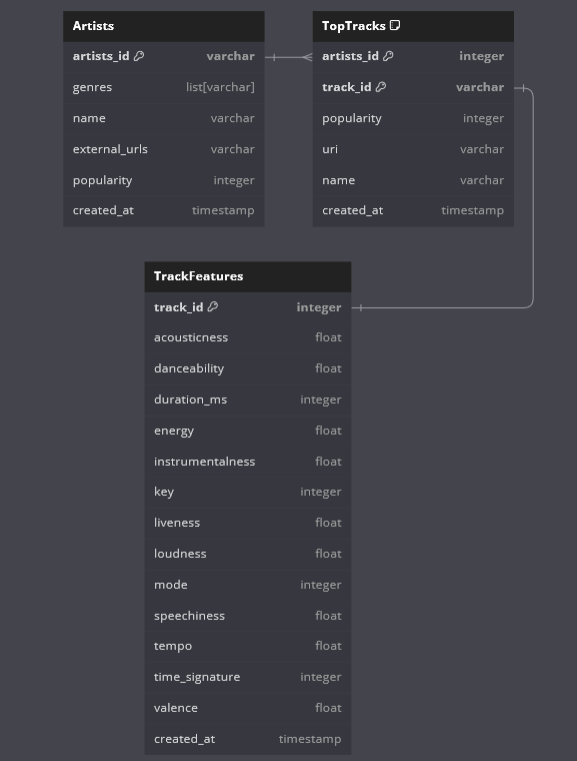
\includegraphics[width=0.5\textwidth]{Basic Relashionship}
  \caption{Estrutura relacional dos dados}
\end{figure}

\section{Treinamento prévio com os dados}

Os algoritmos de aprendizado de máquina usados foram o \textit{Naive Bayes} e \textit{KNN} em \textit{R} para dar dois tipos de classificação uma baseada em metadados e outra baseado em conteúdos, ou seja, a primeira é para recomendar músicas de volume, acústico, duração ou notas parecidas enquanto que a segunda recomendam-se músicas do mesmo gênero, mesmo artista.

Para o treinamento foram usados a informação das tabelas dividindo-os treino e teste na proporção de 70 – 30, 70\% para treino e 30\% para teste, os pesos treinados são localmente armazenados para ambos os algoritmos e utilizado quando o usuário entrar com sua conta do \textit{Spotify}, o fluxo descrito segue o diagrama mostrado na \textit{Figura 2}.

\begin{figure}[h]
  \centering
  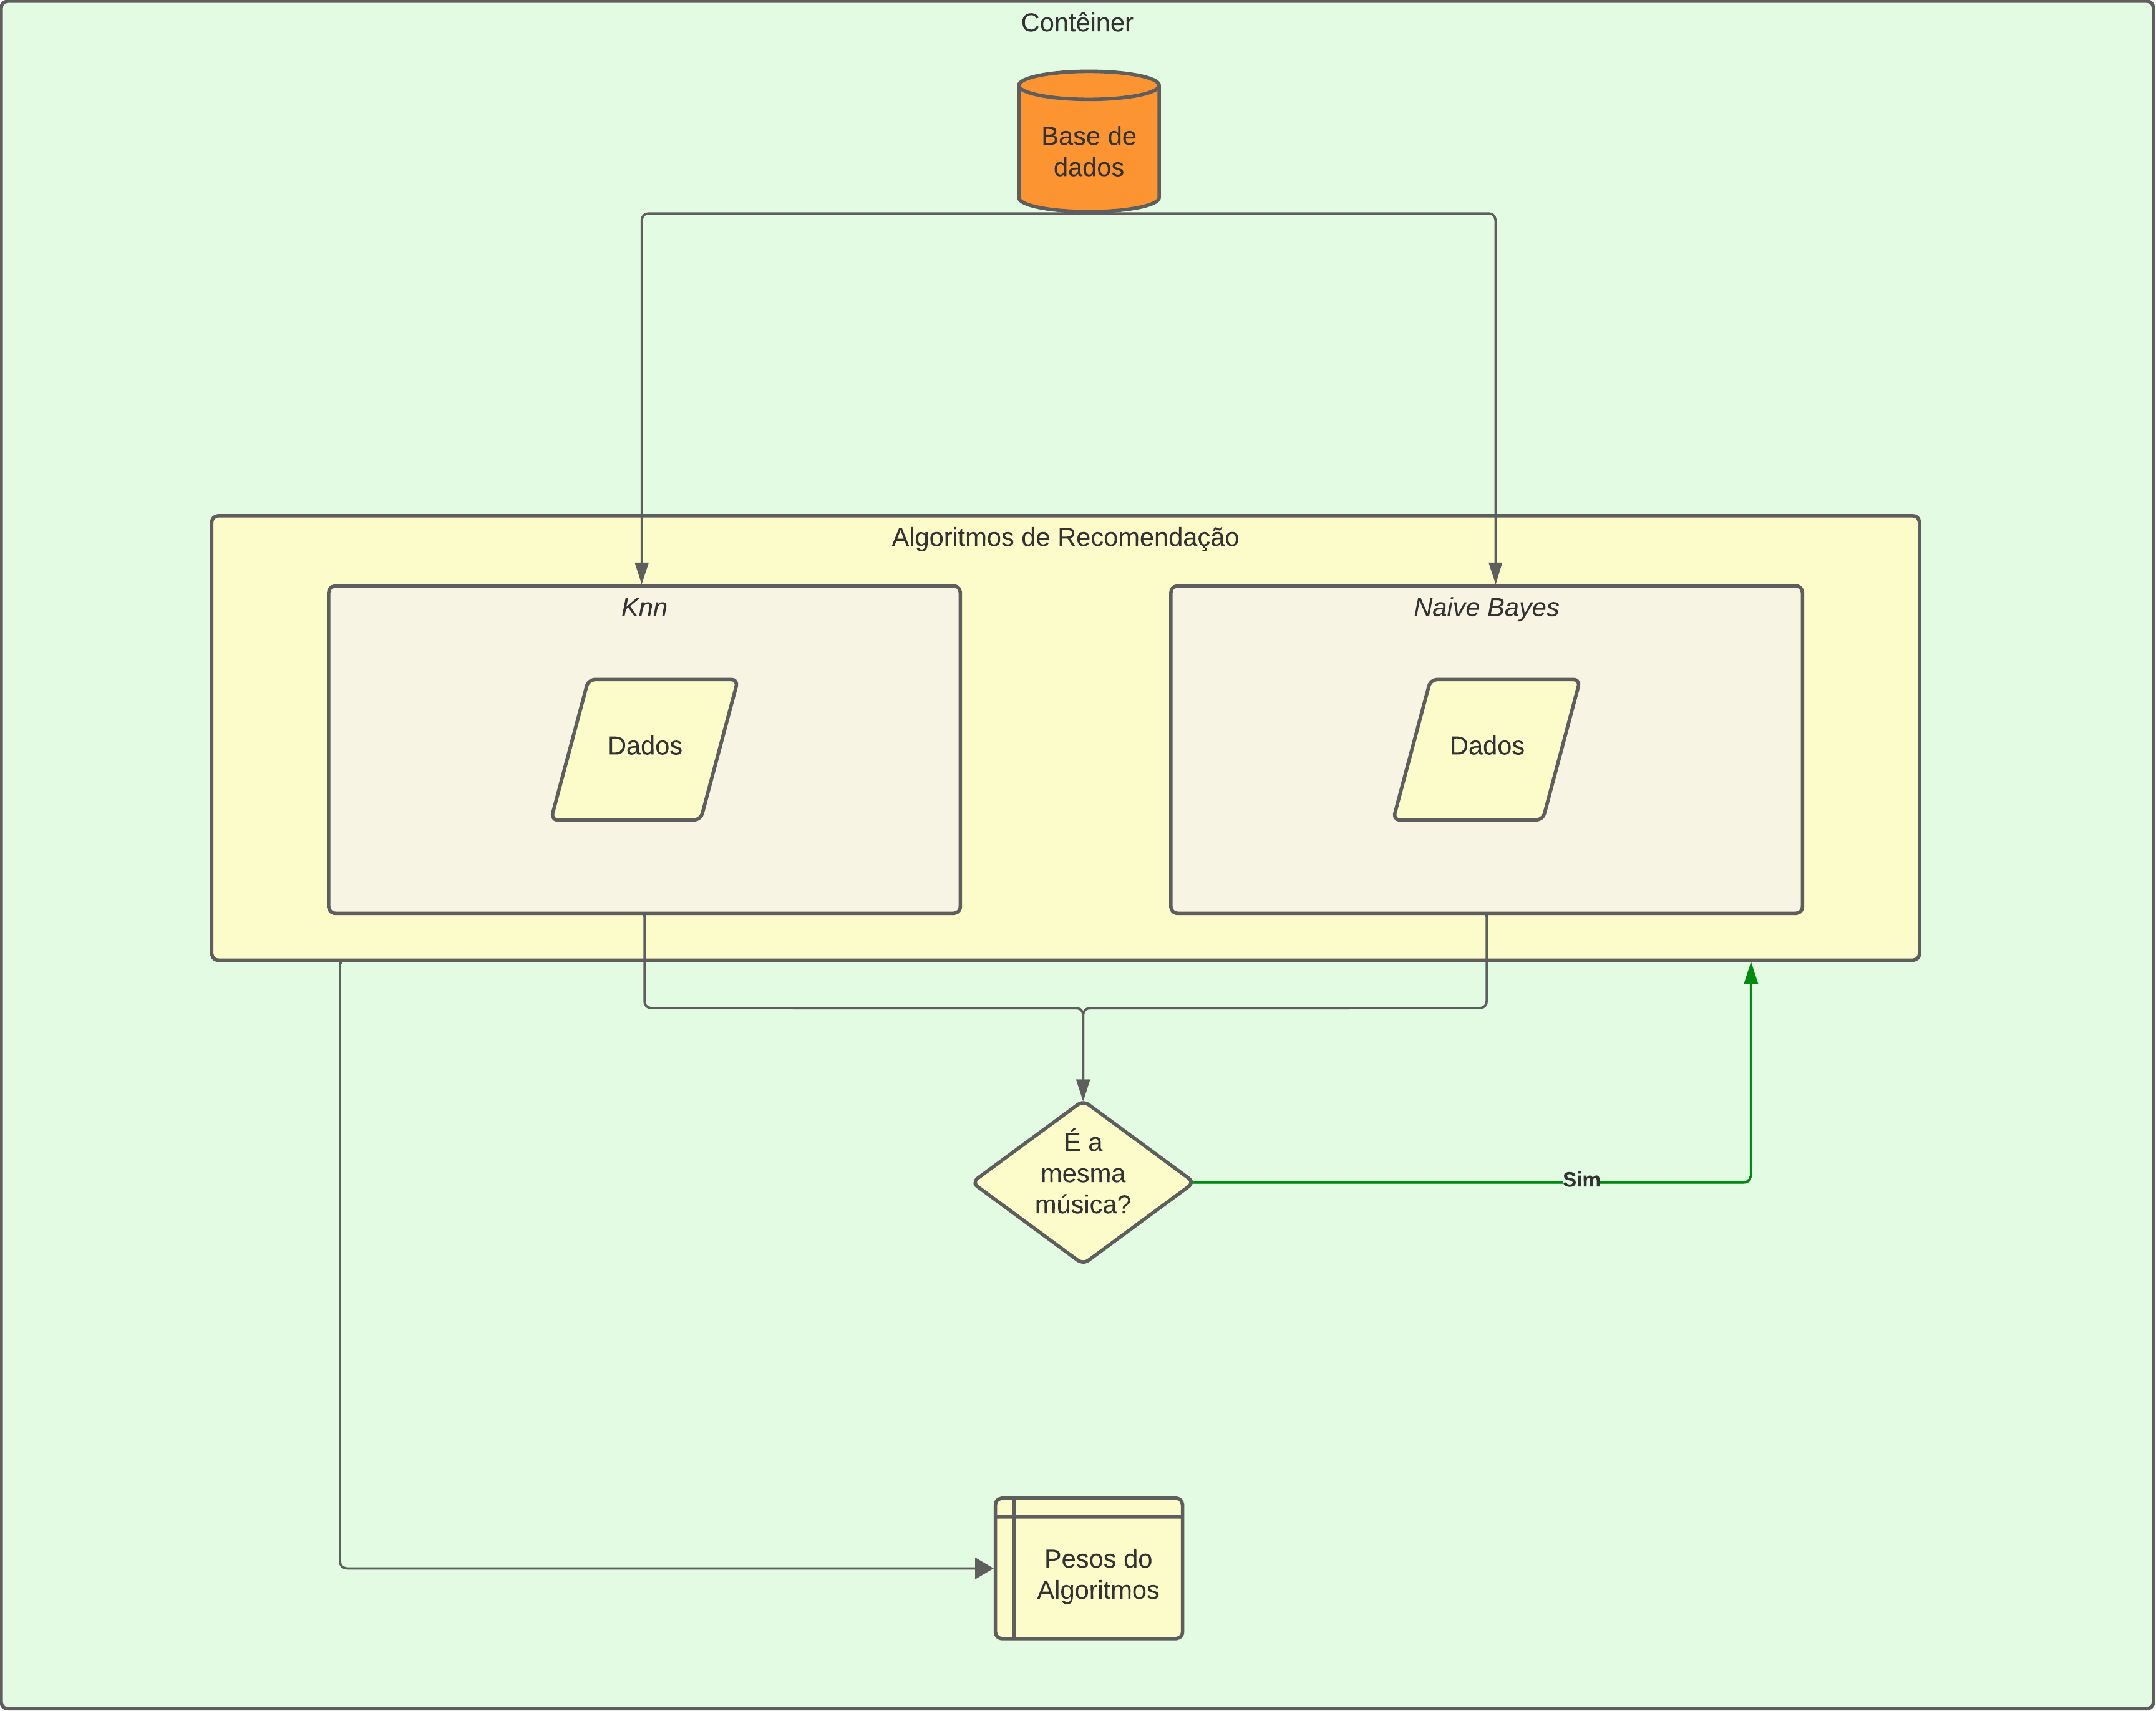
\includegraphics[width=0.5\textwidth]{Diagrama}
  \caption{Fluxo do treinamento prévio}
\end{figure}


\section{Análise do Perfil}

Ao entrar em contato com a interface do sistema o usuário provê com a autorização dele dado cruciais como artistas mais ouvidos, músicas mais tocadas, playlists seguidas e artistas seguidos \cite{SpotifyLink}. Após isso, os pesos do treinamento inicial são carregados e por meio das características dele o modelo prediz músicas que são parecidas com as que ele consome, contudo, não entrou em contato ainda, sendo essa a hipótese da melhor música possível de ser recomendada, e por fim o banco de dados expande-se e o treinamento testa a sua acurácia (explicado na secção 0.4).

Esse processo é mostrado na \textit{Figura 3}, a saída é uma lista de \textit{Uniform Resource Identifier (URI)} das músicas recomendadas, por meio dela o \textit{Spotify} permite a criação de uma playlist dentro do perfil do usuário, onde o usuário pode ouvir, dar uma classificação e um feedback.


\begin{figure}[h]
  \centering
  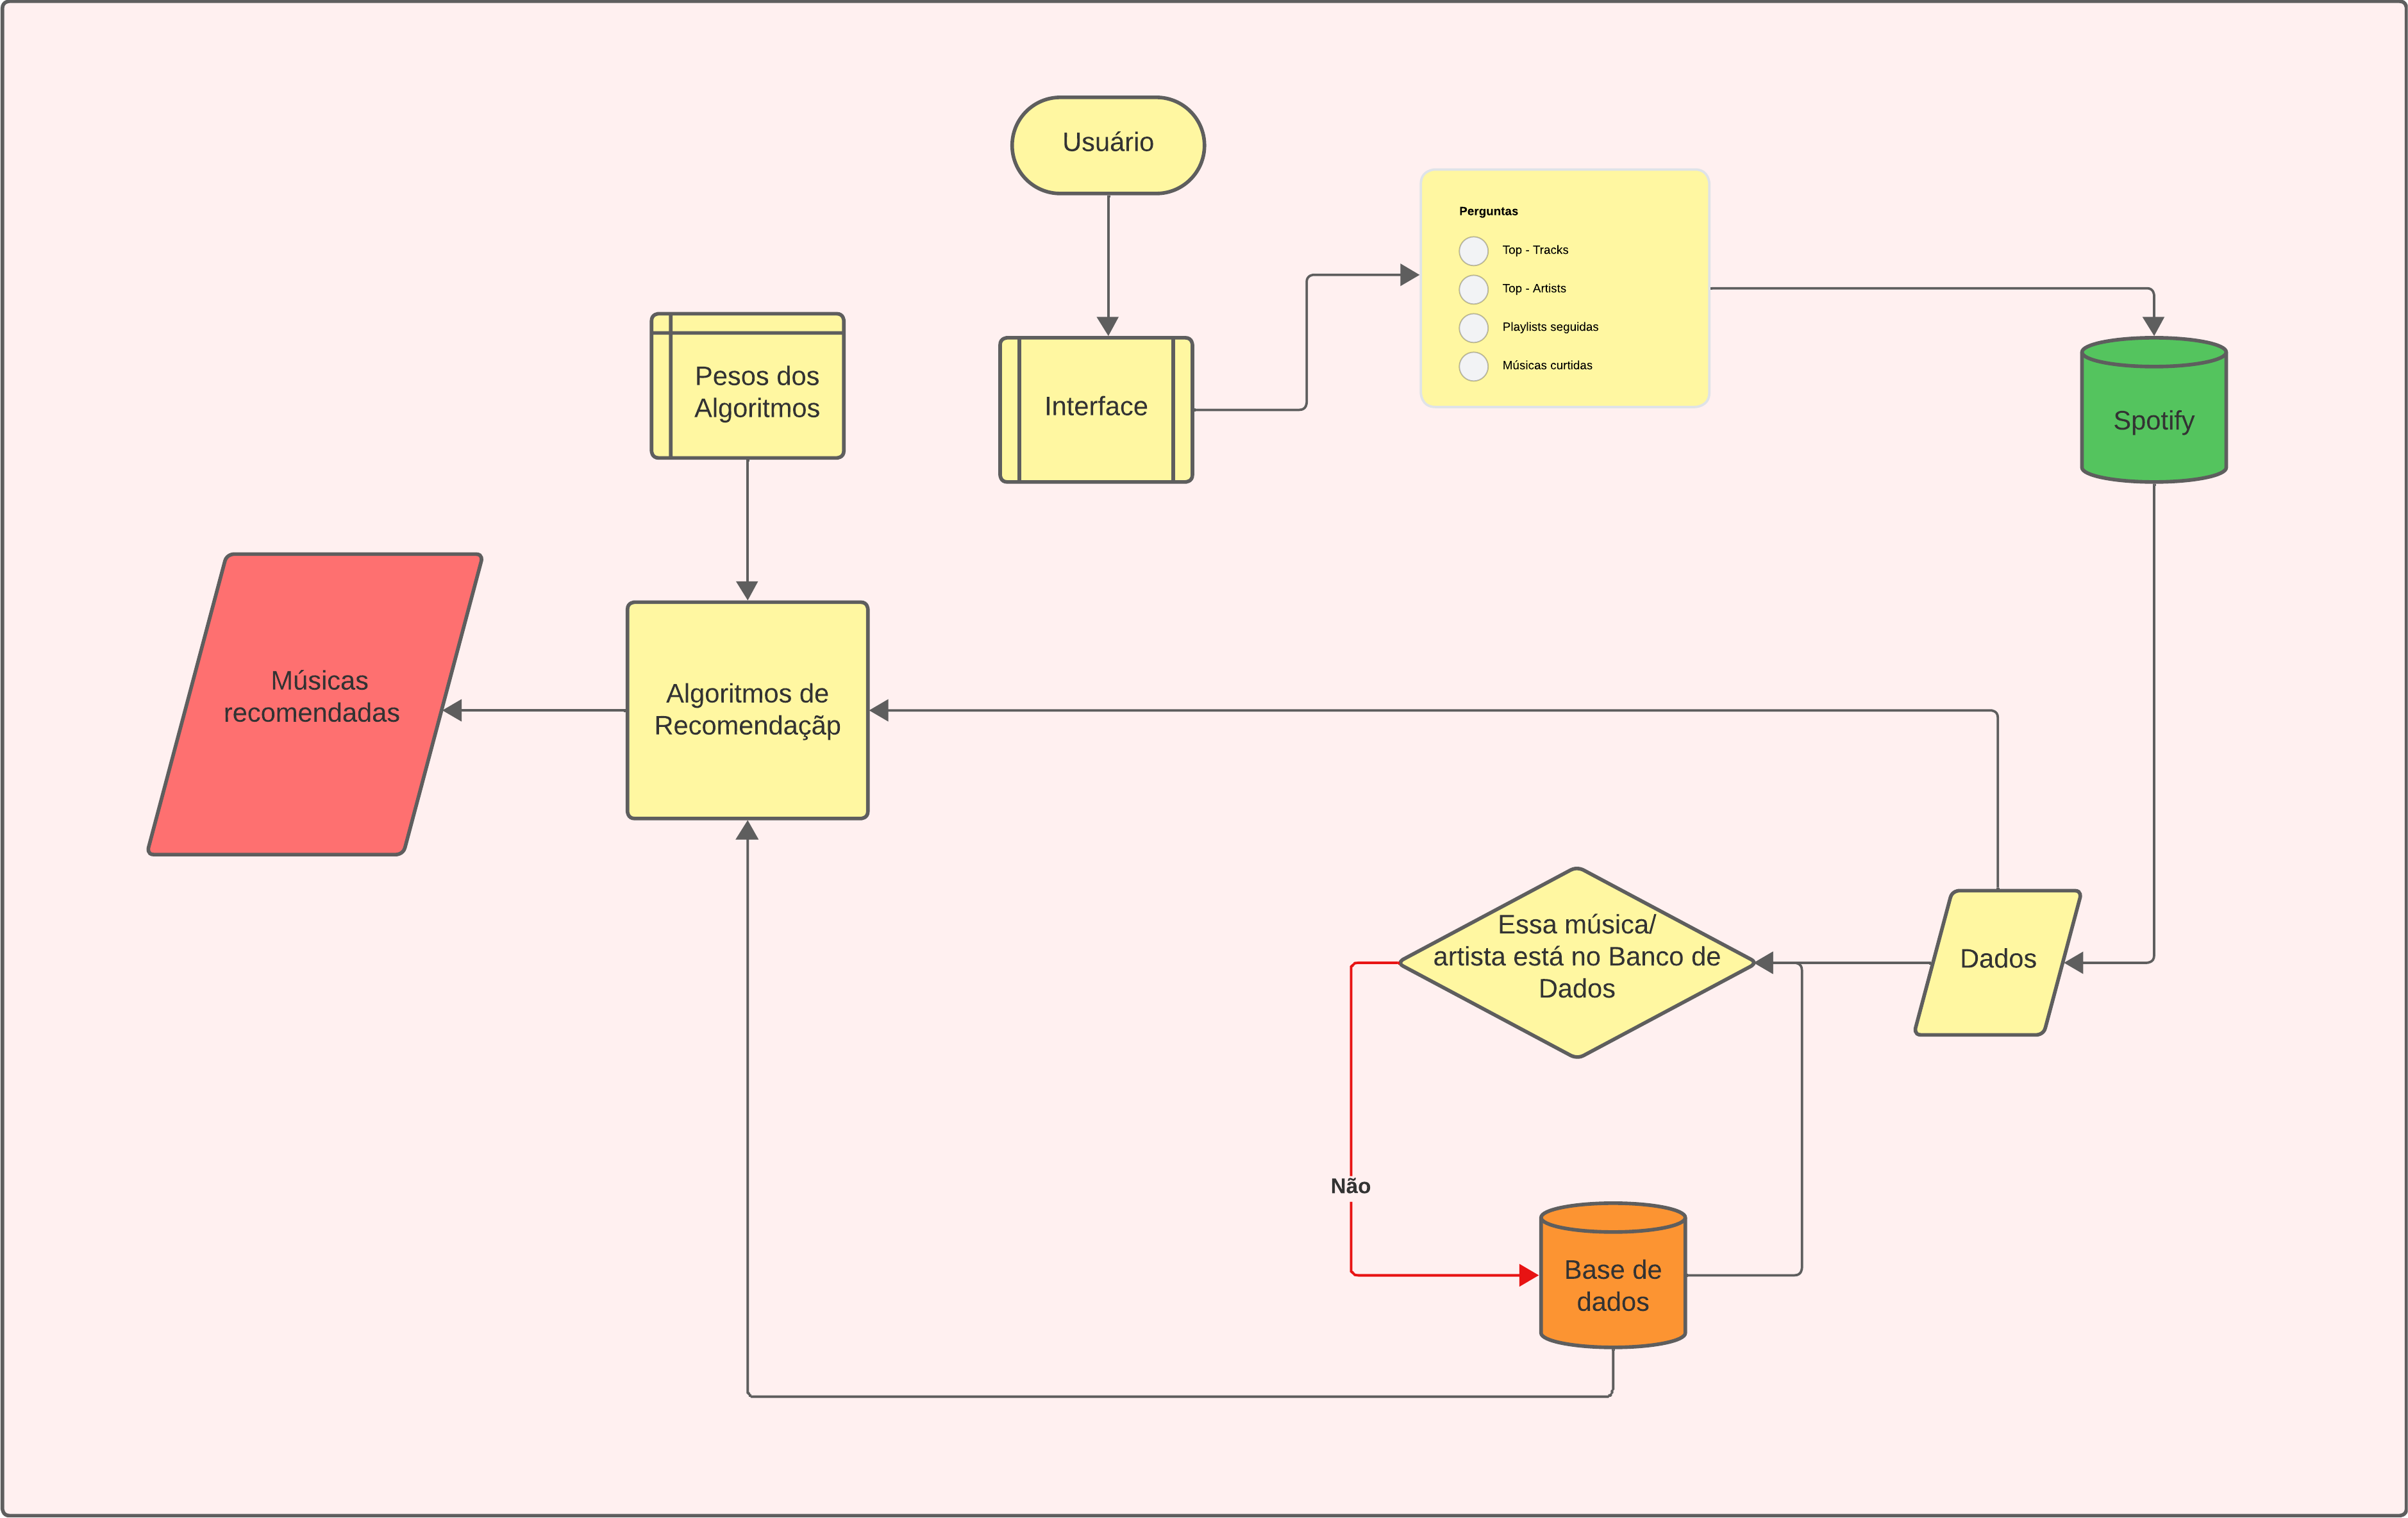
\includegraphics[width=0.5\textwidth]{Diagrama2}
  \caption{Fluxo do contato do cliente}
\end{figure}

\section{Treinamento posterior}

Ao final da comunicação com o cliente, um novo treinamento começa se houver novas características agora com essas músicas e artistas, por fim os pesos são armazenados localmente novamente para serem consumidos para o próximo uso.



\postextual


% ----------------------------------------------------------
% Referências bibliográficas
% ----------------------------------------------------------
\bibliography{abntex2-modelo-references}


%% ----------------------------------------------------------
%% Apêndices TCC: só mantenha se for pertinente.
%% ----------------------------------------------------------

% ---
% Inicia os apêndices
% ---
% \begin{apendicesenv}

% % Imprime uma página indicando o início dos apêndices
% \partapendices

% % ----------------------------------------------------------
% \chapter{Quisque libero justo}
% % ----------------------------------------------------------

% \lipsum[50]

% % ----------------------------------------------------------
% \chapter{Coisas que fiz e que achei interessante mas não tanto para entrar no corpo do texto}
% % ----------------------------------------------------------
% \lipsum[55-57]

% \end{apendicesenv}
% % ---


% % ----------------------------------------------------------
% % Anexos %TCC: so mantenha se pertinente.
% % ----------------------------------------------------------

% % ---
% % Inicia os anexos
% % ---
% \begin{anexosenv}

% % Imprime uma página indicando o início dos anexos
% \partanexos

% % ---
% \chapter{Eu sempre quis aprender latim}
% % ---
% \lipsum[30]

% % ---
% \chapter{Coisas que eu não fiz mas que achei interessante o suficiente para colocar aqui}
% % ---

% \lipsum[31]

% % ---
% \chapter{Fusce facilisis lacinia dui}
% % ---

% \lipsum[32]

% \end{anexosenv}

% %---------------------------------------------------------------------
% % INDICE REMISSIVO
% %---------------------------------------------------------------------

% \printindex



\end{document}